\chapter{Evaluation}

\section{Requirement evaluation}

Concerning the functional requirements, the platform meets the needs by allowing to define data pullers (actors) that incrementally pull various data sources and various resource types.
The pulled data is processed sequentially in a simple pipeline that aggregates, cleans and validates the data before inserting events in the Journal.

Then, the Stream Processing part allows to define a tree of stream processors. A processor can react to events sent by its parent by producing a substream of events towards its children. Substream are inserted in-place in the stream, meaning that the whole substream should be sent to children before processing the next input event. A processor can do a side-effect with a guaranteed exactly-once side-effect semantic, allowing to the user of the library to safely define non-idempotent side-effects.
\\

Concerning the non-functional requirements, all the parts of the architecture are built with an asynchronous non-blocking architecture according to the Reactive Manifesto 
\footfullcite{bib:reactiveManifesto} to optimize performance and resource use by being \textit{event-driven, scalable, resilient and responsive}, the four Reactive Traits.

The Data Integration part is built on top of an Actor system to allow easy concurrency and distribution. Moreover, it makes the best use of resources (CPU, Threads) thanks to a non-blocking implementation. Futures and Iteratees are used to model sequential in-order asynchronous stream processing in a simple, composable and maintainable way. A persistence storage
in MongoDB is used to ensure fault-tolerant pullers: there is no event loss or duplication even in case of failure of a puller. The system is easily distributable 
thanks location transparency that is inherent to the actor model.

The Stream Processing part uses a complex adaptive push-pull model with back-pressure to allow decoupled stream processing while optimizing resource consumption. A stream processor abstraction has been created on top of Iteratees, Futures and Promises. The tree of processors guarantees in-order sequential asynchronous stream processing with fault-tolerance: the temporary failure of a processor is guaranteed without message loss or duplication by allowing a processor to replay the stream from its parent (as shown and explained in section 
\ref{sec:archistream}).


\section{Performance evaluation}

\subsection{Latency and resource consumption}

Performance tests have been performed on the Journal and Stream Processing part on a local machine with a 2.2 GHz processor of 8 cores (so a parallelization factor of 8) with a SSD. The JVM is configured with a maximum Heap size of 2 GB. We will perform tests on the business use case application described in section \ref{sec:usecasebusiness}.
\\

First, we measure the end-to-end latency between the time when an event (1 Ko) is inserted and the time when the resulting dashboard update(s) have been entirely performed. Figure \ref{fig:latencyplot} show the plot of the average end-to-end latency between the Journal and a Dashboard when we increase the push rate of events inserted in the Journal.

We notice that before a threshold of roughly 200 events inserted in the Journal per second, the latency between the Journal and a Dashboard is constant at 4 ms. This means that the processors lower in the tree structure (snapshot, flatSnapshot and the dashboards) can handle the push rate of the Journal and are not late in the stream (push-mode).
However, after 200 events per second, the latency becomes roughly linear with the push rate. This means that dashboards starts to be late in the stream, and are forced to replay events at their rate because their processing time is too slow. Thus, the resultant plot is either constant (up-to-date child processors) or linear (late child processors), which is an expected and good result for scalability.
\\

\begin{figure}
  \begin{center} 
    \makebox[\textwidth]{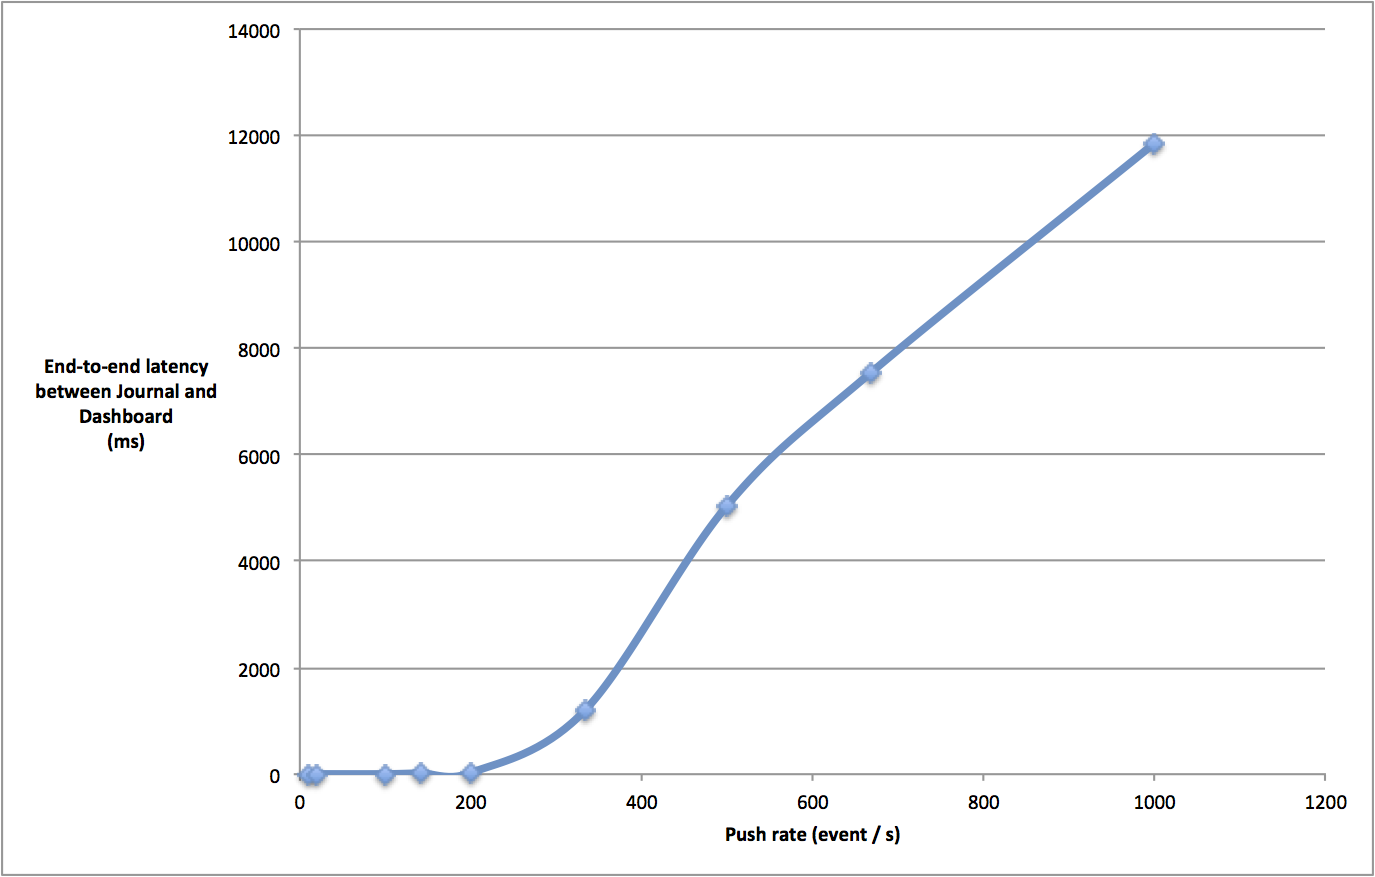
\includegraphics[width=1.0\textwidth]{img/plotlatency.png}}
    \caption{Average latency between the Journal and a Dashboard while varying the Journal push rate}
    \label{fig:latencyplot}
  \end{center}
\end{figure}

To better visualize the fact that low level processors in the tree (dashboards) can catch up with the real-time stream speed or not, Figure \ref{fig:pushrate100}, Figure \ref{fig:pushrate100} and Figure \ref{fig:pushrate1000} shows the latency of each event in sequential order (respectively for Push rate = 100 events / s, Push rate = 500 events / s and Push rate = 1000 events / s). 

We see that in Figure \ref{fig:pushrate100} (100 events / s), almost all events has a latency of 4 ms from the beginning. The peaks of latency that happen sometimes are due to garbage collection. However we notice a higher and slightly larger peak at the beginning of the plot (first events). This is supposed to be due to the initial warmup of the JVM and the components.

On Figure \ref{fig:pushrate500} (500 events / s), we see an initial large latency peak, and then the latency goes back to the normal 4 ms with a few latency peaks due to garbage collection. We notice that the initial latency peak is now larger than in the 100 events / s case. But then, the dashboards manage to catch up with the real-time stream (as their processing speed is still lower than the push rate), and the latency goes back to normal (4 ms) after this warmup time.

However, in Figure \ref{fig:pushrate1000} (1000 events / s), we see that the latency goes on increasing. This is because dashboards do not manage to catch up with the real-time stream that is too fast compared to their processing speed, and so they keep accumulating delay compared to the real-time stream. One solution could be to distribute the dashboards on several machines to allow more resource to them. Moreover, in a real-world scenario, one can hope than times with 1000 events / s are interleaved with moments where the push rate is slower so that the processors have time to reduce their lateness and eventually catch up with the real-time stream. This scenario is simulated in Figure \ref{fig:severalrates}: event 0 to 10000 are pushed with a push rate of 1000 events / s, and just after event 10000 to 20000 are pushed with a push rate of 100 events / s. We see that the processors manages to catch up with the real-time stream around event 12500 and then the latency remains constant at 4 ms.
\\

\begin{figure}
  \begin{center} 
    \makebox[\textwidth]{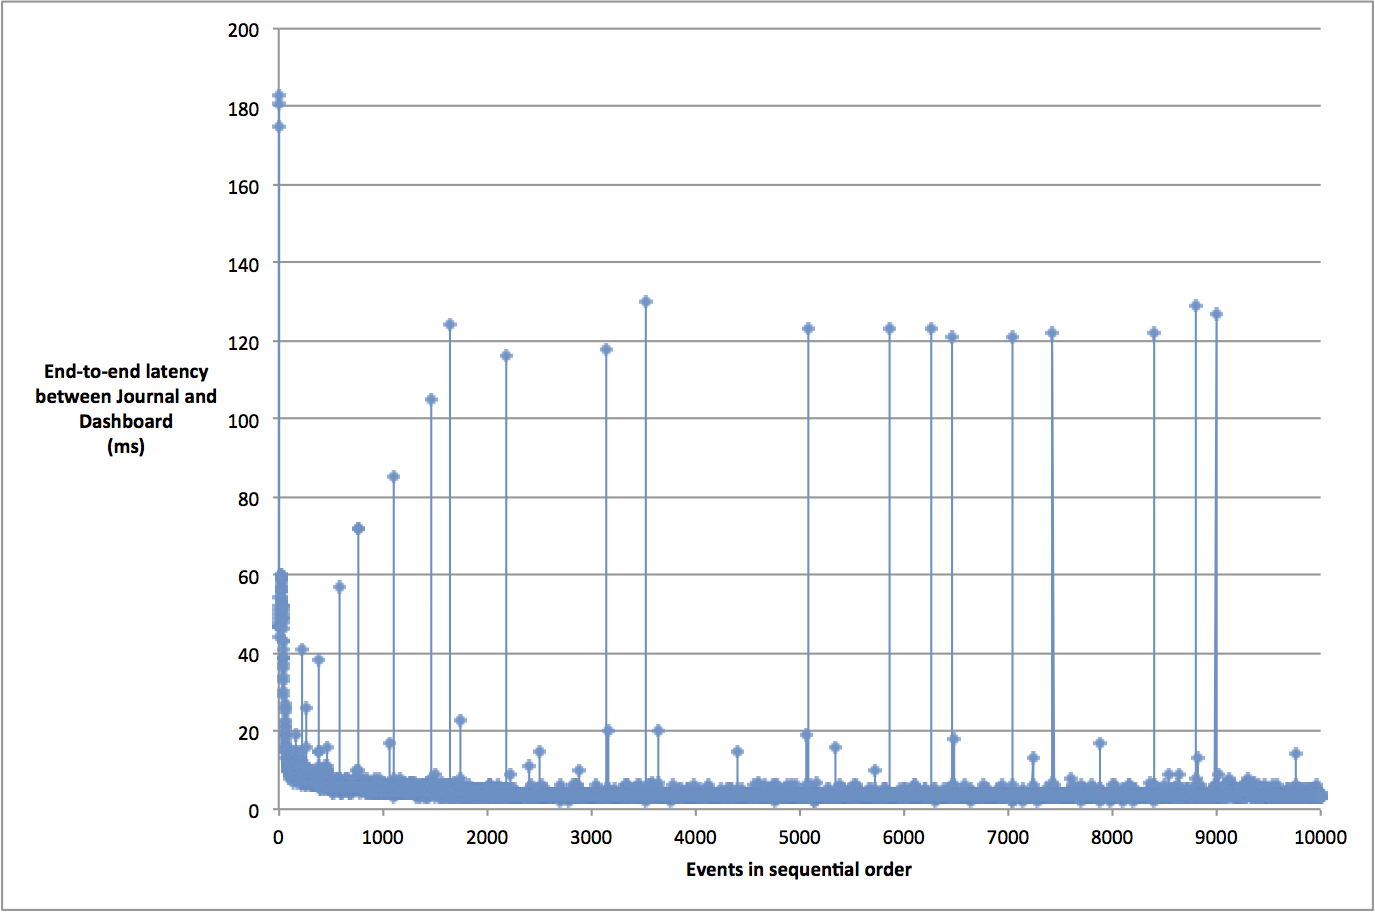
\includegraphics[width=1.0\textwidth]{img/pushrate100.png}}
    \caption{Latency of events between the Journal and a Dashboard with a push rate of 100 events per second}
    \label{fig:pushrate100}
  \end{center}
\end{figure}

\begin{figure}
  \begin{center} 
    \makebox[\textwidth]{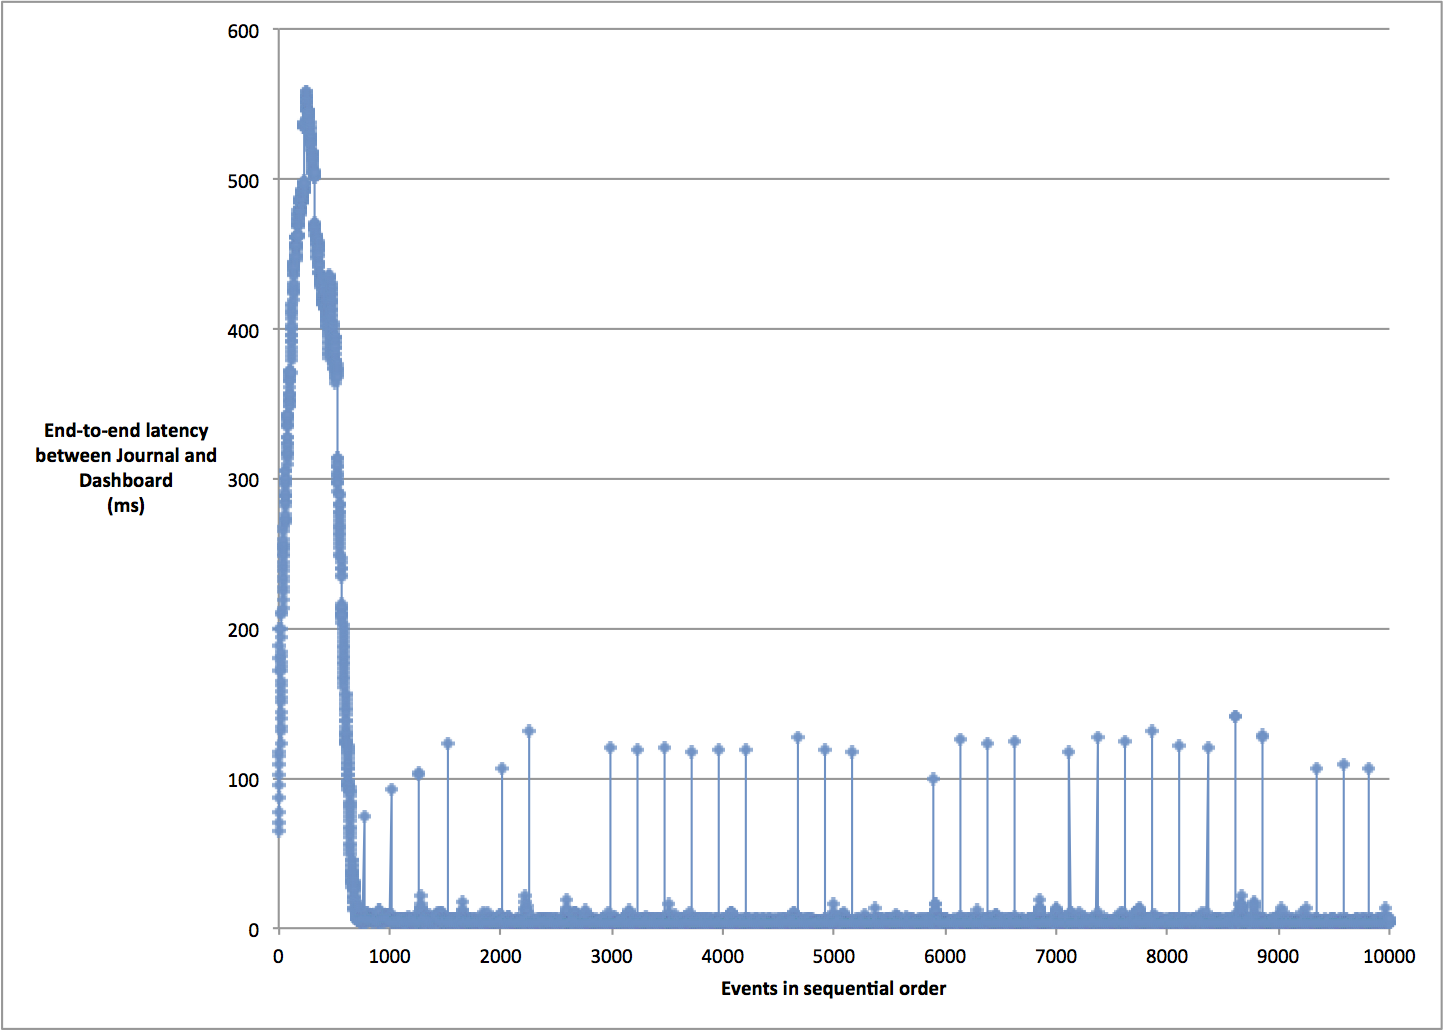
\includegraphics[width=1.0\textwidth]{img/pushrate500.png}}
    \caption{Latency of events between the Journal and a Dashboard with a push rate of 500 events per second}
    \label{fig:pushrate500}
  \end{center}
\end{figure}

\begin{figure}
  \begin{center} 
    \makebox[\textwidth]{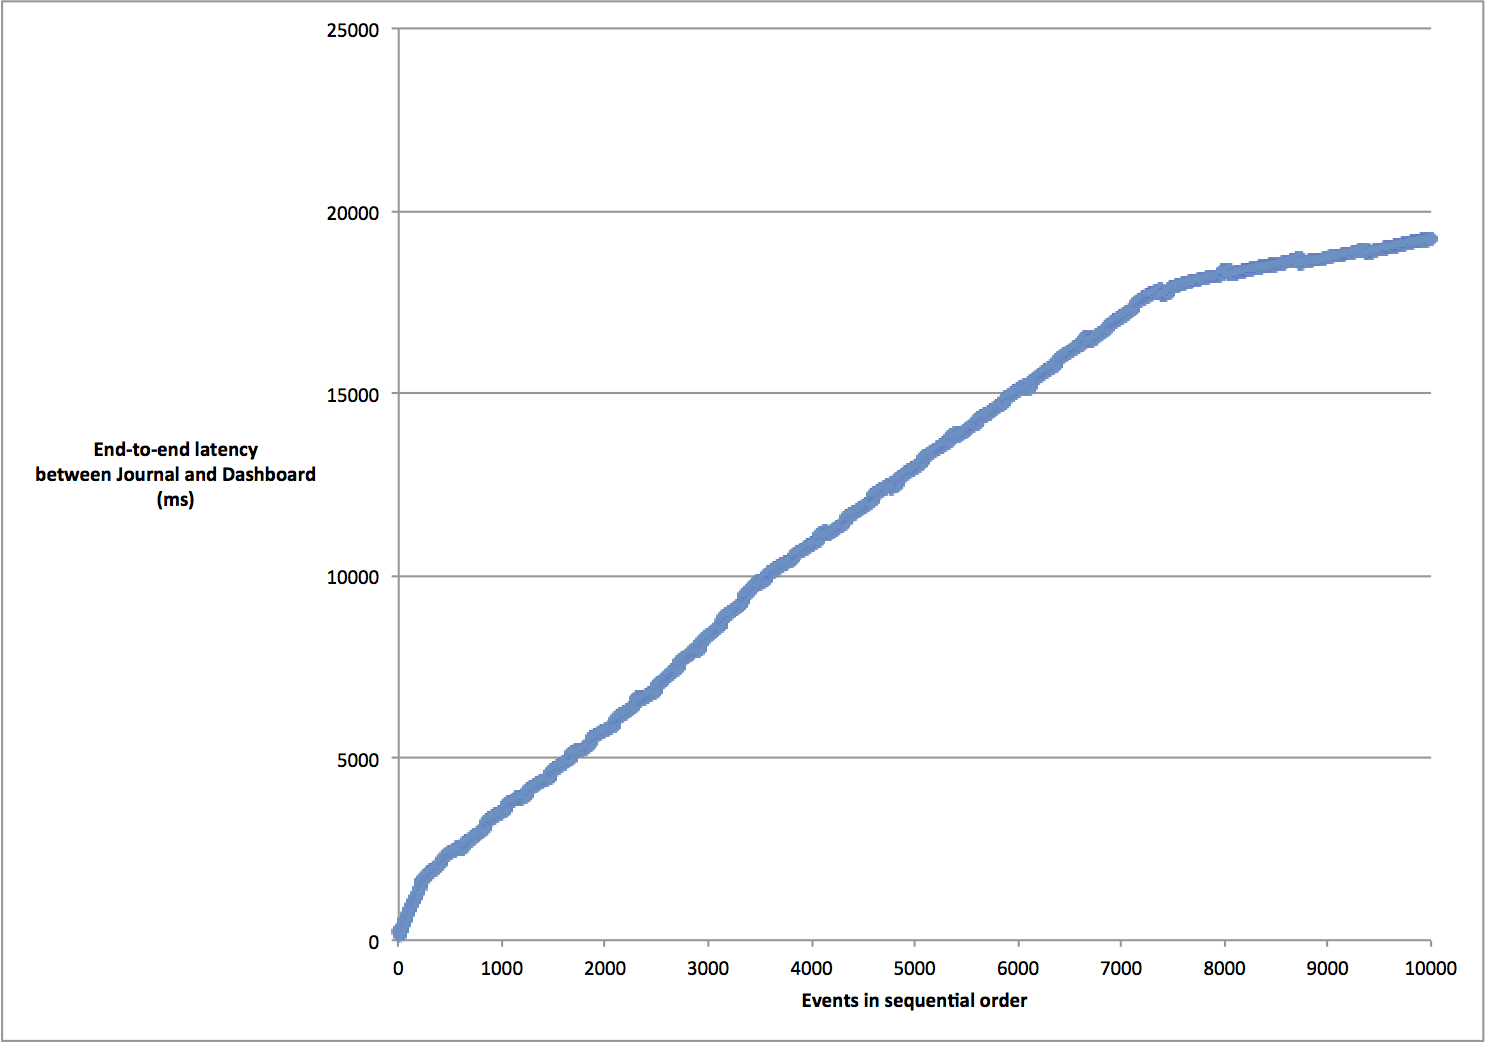
\includegraphics[width=1.0\textwidth]{img/pushrate1000.png}}
    \caption{Latency of events between the Journal and a Dashboard with a push rate of 1000 events per second}
    \label{fig:pushrate1000}
  \end{center}
\end{figure}

\begin{figure}
  \begin{center} 
    \makebox[\textwidth]{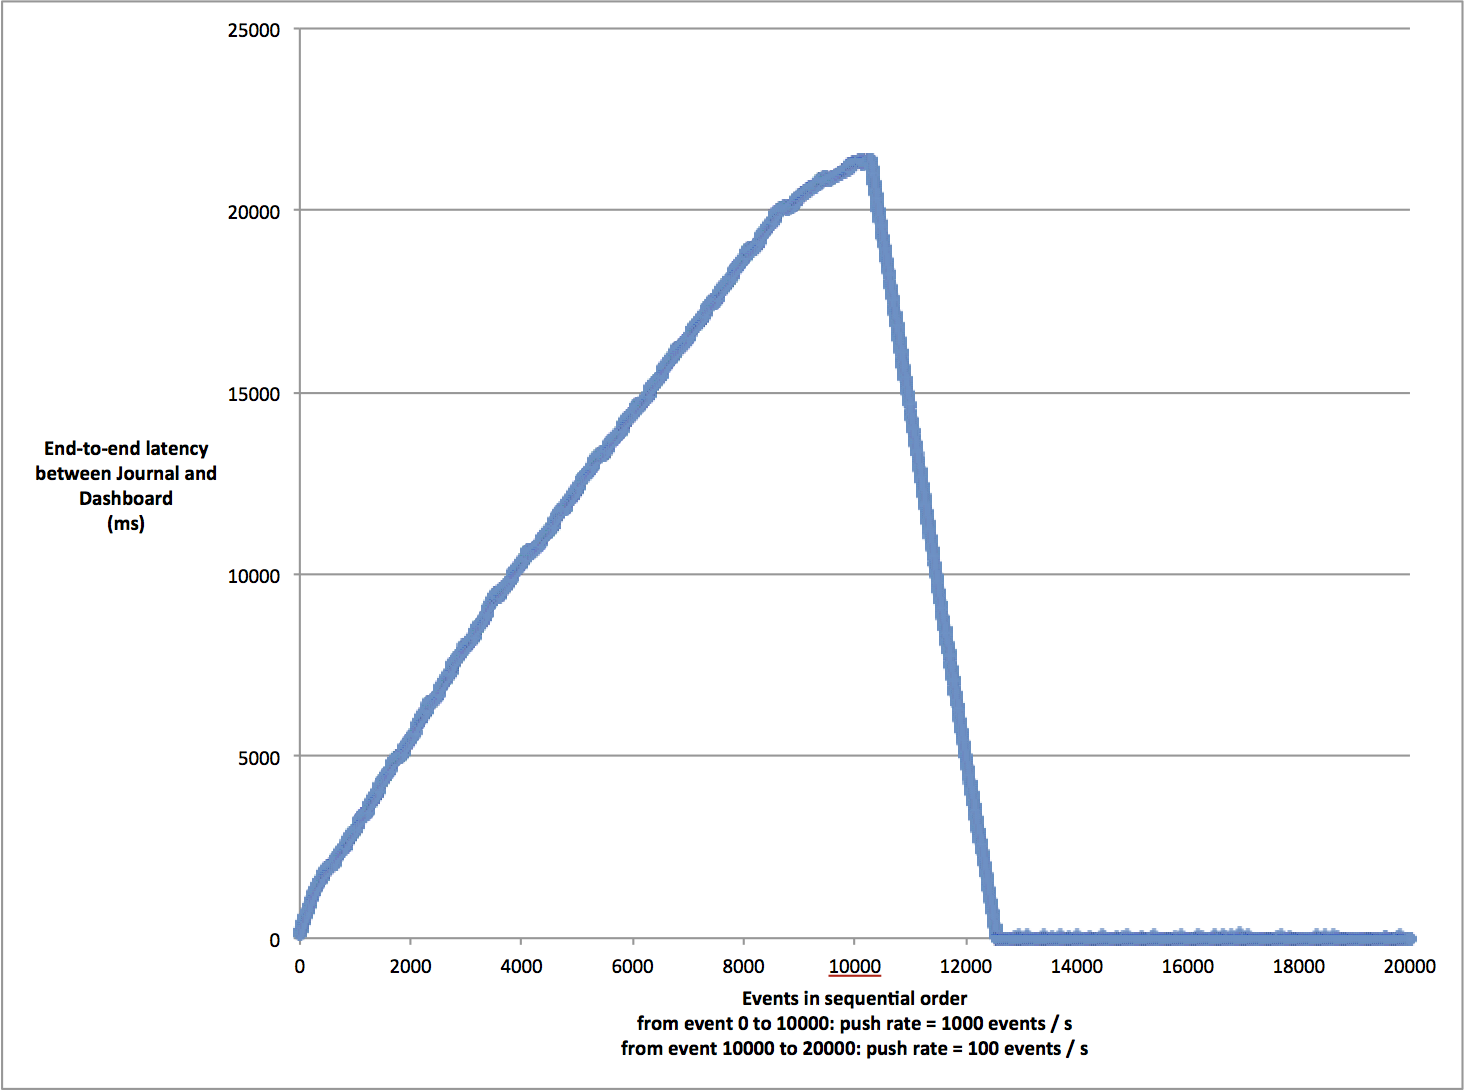
\includegraphics[width=1.0\textwidth]{img/severalrates.png}}
    \caption{Latency of events between the Journal and a Dashboard with variable push rates}
    \label{fig:severalrates}
  \end{center}
\end{figure}


Furthermore, during this performance test, the resource consumption (JVM Heap space, number of threads) has been profiled. Figure \ref{fig:plotheapspace} and Figure \ref{fig:plotthreads} show the JVM Heap space used and the number of threads used while increasing the event push rate on the Journal.
Concerning the number of threads used, we notice that there is a constant number of threads (76) used independently of the push rate, which is expected with our non-blocking IO model to avoid too many context switching.
Concerning the JVM heap space consumption, we notice that the value increase in a less than linear fashion with the push rate (the plot has logarithmic-like shape).
These two plots validate the fact that the platform uses a predictable amount of resource that does not increase too much with the load (optimization of resource consumption).

\begin{figure}
  \begin{center} 
    \makebox[\textwidth]{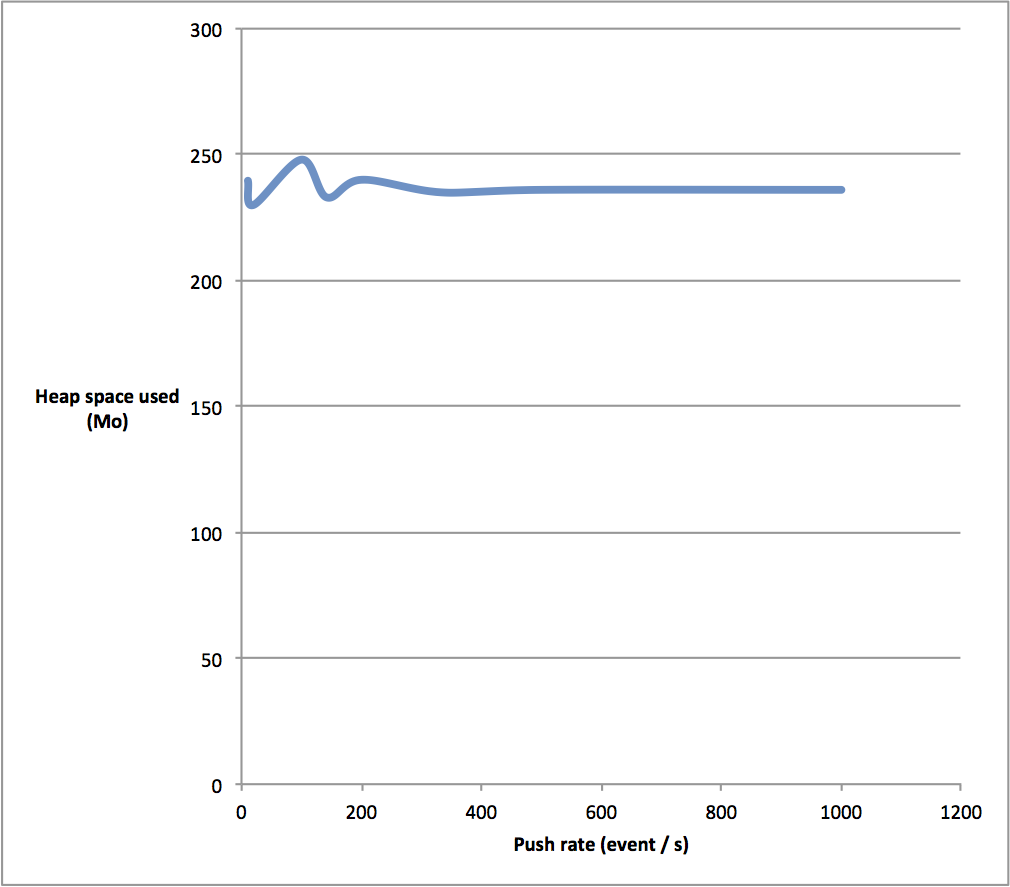
\includegraphics[width=1.0\textwidth]{img/plotheapspace.png}}
    \caption{JVM heap space consumption while varying the Journal push rate}
    \label{fig:plotheapspace}
  \end{center}
\end{figure}

\begin{figure}
  \begin{center} 
    \makebox[\textwidth]{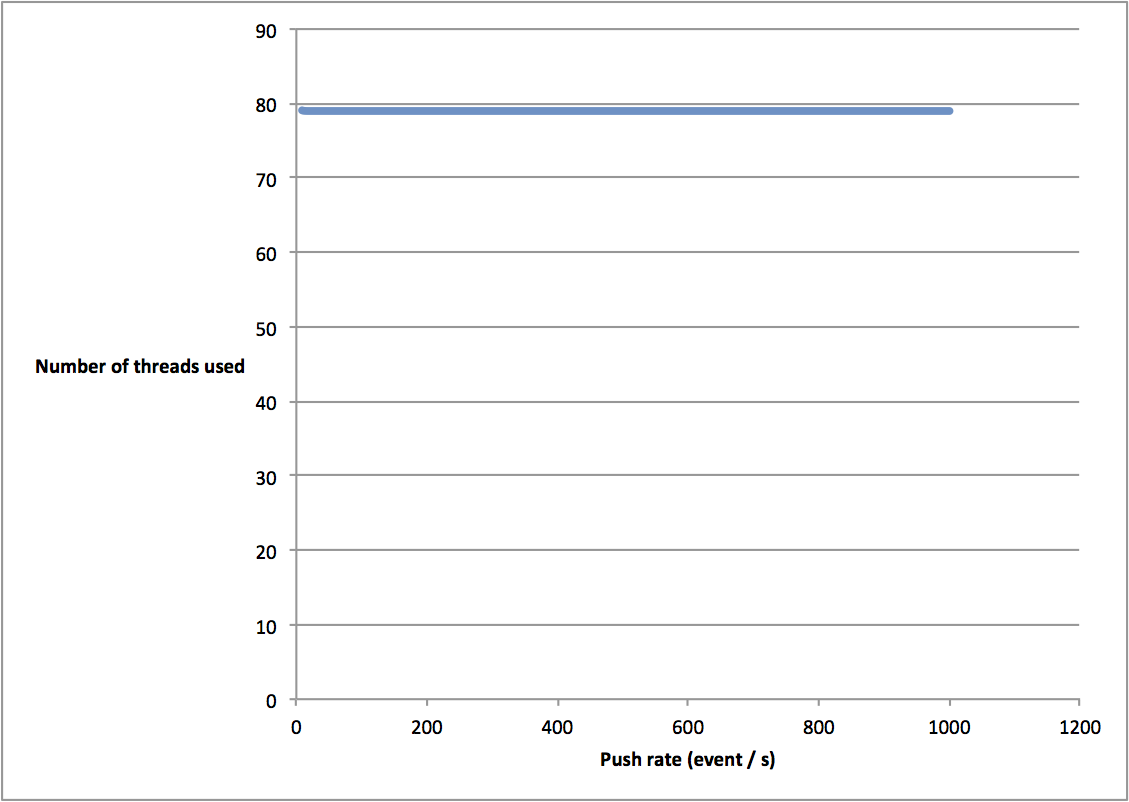
\includegraphics[width=1.0\textwidth]{img/plotthreads.png}}
    \caption{Number of threads used while varying the Journal push rate}
    \label{fig:plotthreads}
  \end{center}
\end{figure}


\subsection{Fault-tolerance}

In this part, we define a performance test to measure the recovery time of a processor that recovers from a crash and must replay 1000 events that happened when it was crashed. Figure \ref{fig:barchart} shows the resultant bar chart.
Using the tree structure of the business use case application presented in section \ref{sec:usecasebusiness}, the Snapshot processor is first killed and then restart. Its parent is the Journal, a persistent processor, so it has only one level to climb in the tree to replay the stream. Then, FlatSnapshot is killed. It is at level 2 in the tree, but its parent is a persistent processor (Snapshot). Therefore, it has also only one level in the tree to climb to replay the stream. As a result, its replay time is roughly the same than Snapshot (the processing time of these two processors is equivalent). Last but not least, a Dashboard is killed. As its parent is a side-effect processor (FlatSnapshot), it has to climb 2 levels to replay the stream (until Snapshot). Moreover, the processing time of a dashboard is slightly superior than other processors. As a result of these two factors (side-effect parent and slightly longer processing time), we see that Dashboard takes more time to replay the 1000 events that it missed, which is expected according to our model.

\begin{figure}[h]
  \begin{center} 
    \makebox[\textwidth]{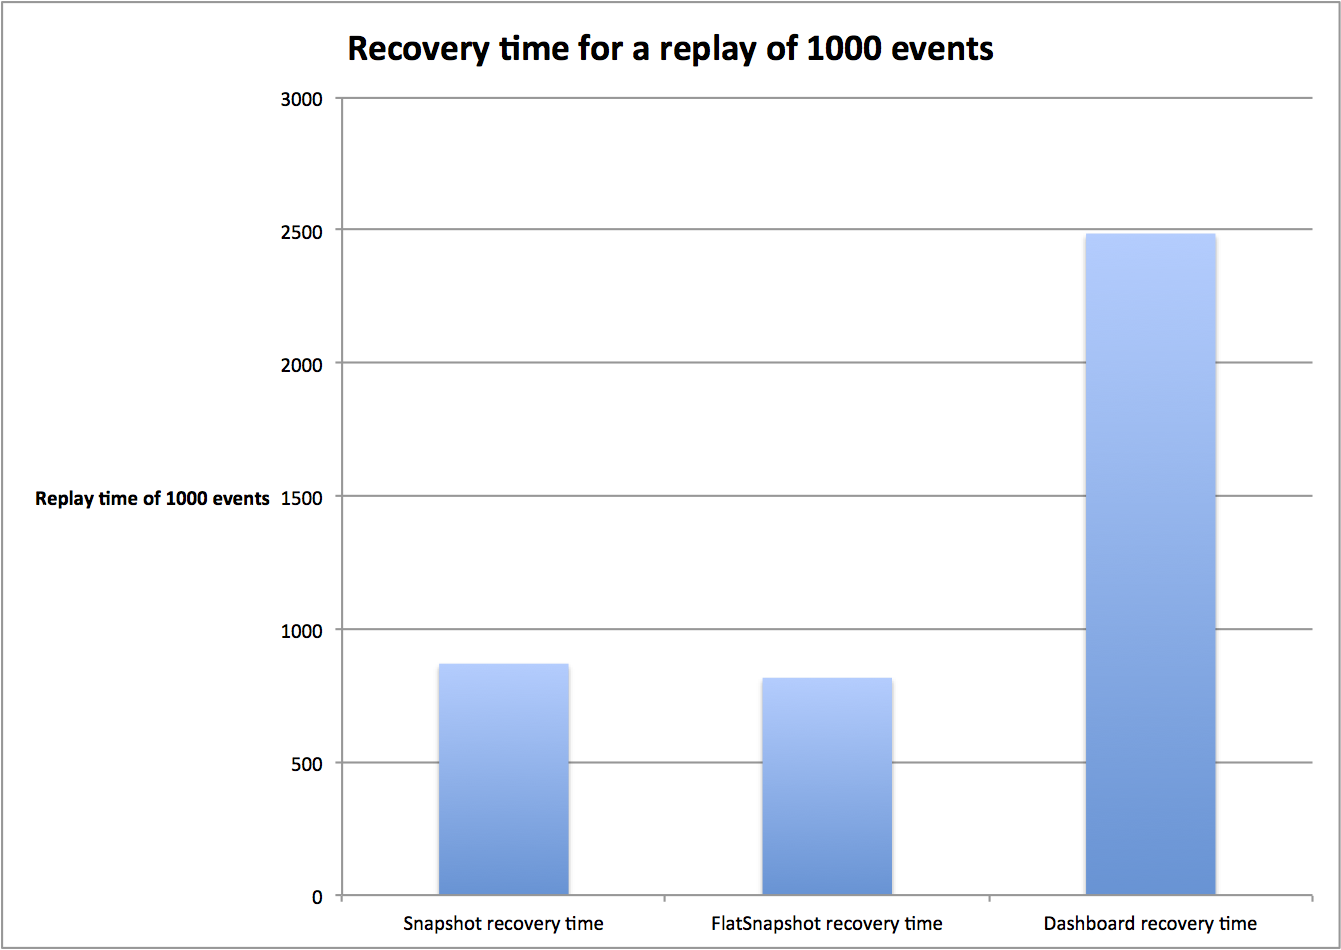
\includegraphics[width=1.0\textwidth]{img/barchart.png}}
    \caption{Recovery time of processors for a replay of 1000 events}
    \label{fig:barchart}
  \end{center}
\end{figure}


